\documentclass[a4paper, 11pt, reqno]{article} % document class(article), paper size (a4paper), font 
                                              % size (12pt), and equation numbering on the right (reqno)
\usepackage{multicol} % for creating multi-column layouts 

\usepackage[T1]{fontenc}  % to use Type 1 fonts for proper embedding

% Mathematical symbols
\usepackage{amsmath,amsfonts,amssymb,amsthm,mathtools} % for formatting and enhancing mathematical notation and equations

% Images
\usepackage{graphicx} % for working with images
\usepackage{tikz} % for creating graphics and diagrams directly 
\usetikzlibrary{calc}
\usepackage{floatrow} % provides additional control over figure and table placement, 
                      % including the [H] option for precise figure placement
\usepackage[margin=10pt,font=small,labelfont=bf,labelsep=period]{caption} % to configure 
                                    % the appearance of captions for figures and tables
%\usepackage{lipsum} % for generating placeholder text

% Tables
\usepackage{array} % for creating arrays and matrices within mathematical environments
\usepackage{tabularx} %  provides an environment for creating tables with columns of 
                      %  varying widths that automatically adjust to fit the content
\usepackage{tabulary} %  similar to the previous one
\usepackage{booktabs} %  enhancing readability and aesthetics
\usepackage{longtable} %  for creating tables that can span multiple pages

% Document's margins
\usepackage[margin=1in]{geometry} % set margins to 1
\geometry{top=25mm}
\geometry{bottom=25mm}
\geometry{left=15mm}
\geometry{right=15mm}

\setlength{\columnsep}{1cm} % set spacing between columns
\setlength{\columnseprule}{0pt} % set rule between columns
\setlength{\parindent}{0pt} % set paragraph indent to zero
\setlength{\parskip}{1ex} % set paragraph spacing

% Algorithms
\usepackage[ruled,vlined]{algorithm2e}

\usepackage{hyperref} % for adding links and customizing them

\usepackage{enumitem} % for itemize adjustment

\usepackage{biblatex} % bibliography-management package
 
\addbibresource{include/references.bib} % Import the bibliography file
\begin{document}
% !TEX root = main.tex

\title[FW Recommendation Systems]{Optimizing Recommendation Systems \\
with the Frank-Wolfe Algorithm}
\subtitle{Optimization for Data Science}
\author[Anna Putina]{Anna Putina\inst{1}}

\institute[Padua]
{
  \inst{1}%
  Università degli Studi di Padova
}

\date[February 5th, 2025] 
{February 5th, 2025}

\logo{
\includegraphics[height=1cm]{image/unipdlogo}}





\newpage

% Abstract section
\section*{Abstract}
\addcontentsline{toc}{section}{Abstract} % Add Abstract to the table of contents 
Recommendation systems are vital tools for providing personalized suggestions to users, enabling them to discover relevant items and enhancing their experience across various domains.  This project explores the application of the Frank-Wolfe algorithm as an effective strategy for recommendation systems. The study is divided into two main parts: a theoretical overview of the Frank-Wolfe algorithm and its mathematical basis, followed by its implementation on two different datasets. The results demonstrate the algorithm’s potential to improve recommendation quality while maintaining computational efficiency across diverse datasets.
\vspace{1cm}

%\newpage
%\tableofcontents{}

%\newpage
\begin{multicols}{2} % start two-column layout


\section{Introduction}

Recommendation systems play an essential role in various digital platforms by predicting user preferences and delivering personalized suggestions. These systems operate on data that typically involves three key components: users, items, and ratings. Ratings, either explicit (e.g., star ratings) or implicit (e.g., clicks or views), are used to model user preferences. The ultimate goal is to predict unknown ratings or preferences for items that a user has not yet interacted with, enabling the system to recommend the most relevant content. This task is inherently challenging due to the sparsity of the data—most users rate or interact with only a small subset of the available items—and the need to balance accuracy with computational efficiency.

To address these challenges, this project investigates the use of the Frank-Wolfe algorithm, a first-order optimization method, to enhance the performance of recommendation systems. The Frank-Wolfe algorithm \cite{Frank1956AnAF} is well-regarded for its simplicity, efficiency, and ability to handle large-scale problems with constraints. Its iterative process, which involves solving a linear subproblem at each step, makes it computationally light compared to second-order methods. Furthermore, its tendency to produce sparse solutions aligns naturally with the sparse structure of recommendation system data, making it an attractive choice for this context.

The project is divided into two main parts. The first part focuses on the theoretical foundation of the Frank-Wolfe algorithm, providing an in-depth explanation of its mathematical formulation and discussing its strengths and limitations in the context of recommendation systems. The second part applies the algorithm to real-world recommendation system datasets to evaluate its practical performance. By analyzing prediction accuracy and computational efficiency, this project seeks to demonstrate the utility of the Frank-Wolfe algorithm as an effective optimization technique for modern recommendation systems.


\section{The Frank-Wolfe Algorithm}

The Frank-Wolfe algorithm, also known as the conditional gradient method, is a first-order optimization technique for solving constrained convex optimization problems. It is particularly effective when the feasible region is convex and the solution is sparse. The algorithm avoids computationally expensive projections onto the feasible region by instead solving a linear subproblem at each iteration using a Linear Minimization Oracle (LMO).

The LMO is a key component of the algorithm, defined as:
\[
\text{LMO}_C(\nabla f(x)) = \arg\min_{s \in C} \langle \nabla f(x), s \rangle,
\]
where \(C\) is the feasible region, and \(\nabla f(x)\) is the gradient of the objective function at the current iterate \(x\). The LMO identifies a point \(s_k\) in the feasible region that minimizes the linear approximation of the objective function, guiding the update direction.

Given a convex objective function \(f(x)\) and a convex feasible region \(C\), the algorithm solves:
\[
\min_{x \in C} f(x).
\]

The pseudocode for the Frank-Wolfe algorithm is presented below:

\begin{algorithm}[H]
\caption{Frank-Wolfe Method}
\KwIn{Convex function \(f(x)\), feasible region \(C\), initial point \(x_0 \in C\)}
\For{\(k = 0, 1, \dots\)}{
    Compute \(s_k = \arg\min_{s \in C} \langle \nabla f(x_k), s \rangle\) using LMO\;
    Set direction \(d_k^{FW} = s_k - x_k\)\;
    Choose step size \(\alpha_k \in (0, 1]\)\;
    Update \(x_{k+1} = x_k + \alpha_k d_k^{FW}\)\;
    \If{stopping condition is met}{break\;}
}
\end{algorithm}

\section{Using Frank-Wolfe for Matrix Completion}

Matrix completion is one way to apply the Frank-Wolfe algorithm to recommendation systems. In recommendation systems, the idea is to predict missing entries in a user-item interaction matrix \(X\), where rows represent users, columns represent items, and the values represent user ratings or interactions. This matrix is usually very sparse since most users interact with only a small number of items.

The goal is to retrieve a low-rank matrix \(X \in \mathbb{R}^{n_1 \times n_2}\) from a sparse set of observed matrix entries \(\{U_{ij}\}_{(i,j) \in J}\), where \(J \subset [1:n_1] \times [1:n_2]\). The problem can be formulated as follows\cite{doi:10.1137/15M104726X}:

\[
\min_{X \in \mathbb{R}^{n_1 \times n_2}} f(X) := \sum_{(i,j) \in J} (X_{ij} - U_{ij})^2, \\
\text{s.t.} \quad \text{rank}(X) \leq \delta,
\]


where the function \(f\) is the squared loss over the observed entries of the matrix, and \(\delta > 0\) is a parameter representing the assumed belief about the rank of the reconstructed matrix. In practice, the low-rank constraint is relaxed with a nuclear norm ball constraint (the nuclear norm \(\|X\|_*\) of a matrix \(X\) is equal to the sum of its singular values). Thus, we get the following convex optimization problem:

\[
\min_{X \in \mathbb{R}^{n_1 \times n_2}} \sum_{(i,j) \in J} (X_{ij} - U_{ij})^2, \quad \text{s.t.} \quad \|X\|_* \leq \delta.
\]

The feasible set is the convex hull of rank-one matrices:
\[
\begin{aligned}
C = \{X \in \mathbb{R}^{n_1 \times n_2} : \|X\|_* \leq \delta\} \\
= \text{conv}\{\delta uv^\top : u \in \mathbb{R}^{n_1}, v \in \mathbb{R}^{n_2}, \|u\|_2 = \|v\|_2 = 1\}.
\end{aligned}
\]



If we indicate with \(A_J\) the matrix that coincides with \(A\) on the indices \(J\) and is zero otherwise, then we can write:
\[
\nabla f(X) = 2 (X - U_J).
\]

Thus, we have the following LMO in this case:
\[
\text{LMO}_C(\nabla f(X_k)) \in \arg\min \{\text{tr}(\nabla f(X_k)^\top X) : \|X\|_* \leq \delta\},
\]

which boils down to computing the gradient and the rank-one matrix \(\tau u_1 v_1^\top\), where \(u_1, v_1\) are the right and left singular vectors corresponding to the top singular value of \(-\nabla f(X_k)\). Consequently, the Frank-Wolfe method at a given iteration approximately reconstructs the target matrix as a sparse combination of rank-one matrices. Furthermore, as the gradient matrix is sparse (it only has \(|J|\) non-zero entries), storage and approximate singular vector computations can be performed much more efficiently than for dense matrices.

\section{Datasets}

To evaluate the performance of the Frank-Wolfe algorithm for matrix completion in recommendation systems, two different datasets were used. 

\subsection{MovieLens 20M Dataset}
The first dataset\cite{10.1145/2827872} used in this project is the MovieLens 20M dataset, a widely recognized benchmark in recommendation systems research. This dataset contains 20 million ratings provided by 138,000 users for over 27,000 movies. Each rating ranges from 0.5 to 5.0 and includes metadata such as movie titles, genres, and timestamps.

\subsection{Anime User Score Dataset}
The second dataset\cite{animeDataset} focuses on the anime domain. This dataset contains user ratings for 16,500 anime titles, provided by 270,033 users. By leveraging these scores, the dataset enables the development of recommendation systems that align with individual tastes. The Anime User Score dataset presents unique challenges, such as a highly diverse user base and varying item popularity, making it a complementary addition to the MovieLens dataset for testing the Frank-Wolfe algorithm. 

Both datasets were used to test the algorithm's ability to handle large, sparse matrices and to evaluate its performance in predicting missing ratings. 

\section{Implementation Details}

The implementation of the Frank-Wolfe algorithm for matrix completion was designed to ensure meaningful results and make the algorithm efficient\cite{d8e5ac9d80b841129c2d1ff124cda213}. Below, we outline the key aspects of the implementation.

\subsection{Dataset Preparation}
To maintain proper sparsity in the datasets, only a subset of the data was used for testing. Specifically, we focused on 20-50\% of the available data, ensuring that the observed entries represented a realistic level of sparsity commonly found in recommendation systems. Additionally, we prioritized active users (those with a sufficient number of ratings) and popular products (those with a high number of ratings) to improve the reliability of the results.

\subsection{Algorithm Tracking and Stopping Criteria}
The algorithm was designed to monitor several key metrics during its execution:
\begin{itemize}
    \item \textbf{Loss Function}: The loss function \(f(X)\) is the squared error over the observed entries:
    \[
    f(X) = \sum_{(i,j) \in J} (X_{ij} - U_{ij})^2.
    \]
    \item \textbf{Dual Gap}: The dual gap is a measure of suboptimality and is used as a stopping criterion. It is defined as:
    \[
    \text{Dual Gap} = \langle \nabla f(X_k), X_k - S_k \rangle,
    \]
    where \(S_k\) is the solution provided by the Linear Minimization Oracle (LMO) at iteration \(k\). A smaller dual gap indicates that the current solution is closer to the optimal solution.
    \item \textbf{Relative Change Between Iterates}: The relative change between matrices in two subsequent iterations is computed as:
    \[
    \frac{\|X_{k+1} - X_k\|_F}{\|X_k\|_F}.
    \]
    This metric ensures that the algorithm terminates when updates to the solution become negligible.
\end{itemize}
Any of these parameters can be used as stopping criteria, with thresholds chosen to balance accuracy and computational efficiency.

\subsection{Learning Rate Strategies}
Several learning rate strategies were implemented to determine the step size \(\alpha_k\) at each iteration:
\begin{itemize}
    \item \textbf{Diminishing Step Size}: This is the standard step size for Frank-Wolfe, defined as:
    \[
    \alpha_k = \frac{2}{k + 2}.
    \]
    \item \textbf{Exact Line Search}: The step size is chosen to minimize the loss function along the update direction:
    \[
    \alpha_k = \arg\min_{\alpha \in [0, 1]} f(X_k + \alpha (S_k - X_k)).
    \]
    \item \textbf{Armijo Rule}: The step size satisfies the Armijo condition:
    \[
    f(X_k + \alpha_k d_k) \leq f(X_k) + c \alpha_k \langle \nabla f(X_k), d_k \rangle,
    \]
    where \(d_k = S_k - X_k\) is the update direction, and \(c \in (0, 1)\) is a pre-defined constant.
\end{itemize}

\subsection{Performance Tracking}
The performance of the algorithm was evaluated by tracking the loss function and the dual gap across iterations. These metrics provide insights into the convergence of the algorithm and the quality of the solution. The final results include a comparison of the loss and dual gap for different learning rate strategies, showcasing the effectiveness and efficiency of the Frank-Wolfe algorithm for matrix completion.


\section{Results}

After running the Frank-Wolfe algorithm on the two datasets, we observed significant differences in the performance of the various learning rate strategies. Specifically, the simplest learning rate strategy, the diminishing step size, resulted in lower performance compared to the other methods for the same number of iterations (800 iterations in our experiment). However, it is the fastest method in terms of computational time. 

In contrast, the more advanced strategies, such as exact line search and the Armijo rule (faster than exact line search in terms of iterations), showed much better performance. However, exact line search is the slowest method in terms of computational time. These methods resulted in better convergence and lower final loss values, demonstrating their suitability for this problem.



\begin{figure}[H]
    \centering
    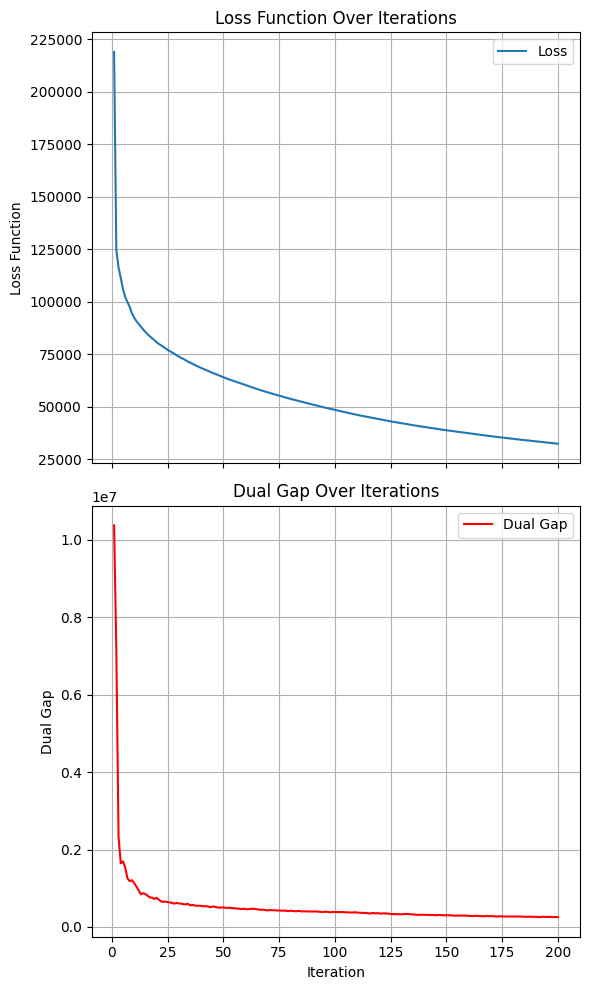
\includegraphics[width=0.8\textwidth]{images/movielens_loss_gap}
    \caption{Loss function and dual gap vs iterations for the MovieLens 20M dataset.}
    \label{fig:movielens}
\end{figure}

The results are illustrated in the following plots (Figures~\ref{fig:movielens} and \ref{fig:anime}), which show the loss function and dual gap versus the number of iterations for both the MovieLens 20M dataset and the Anime User Score dataset. These plots are created implementing the exact line search strategy.

To evaluate performance, we computed the relative accuracy function, which measures the percentage of predictions that fall within a given tolerance of the true values. The results of this evaluation are summarized in the table below.

\begin{table}[H]
    \centering
    \begin{tabular}{|c|c|c|}
        \hline
        \textbf{Dataset} & \textbf{Step Size} & \textbf{ Accuracy (\%)} \\ \hline
        MovieLens & Diminishing & 62 \\ \hline
        MovieLens & Line Search & 82 \\ \hline
        MovieLens & Armijo & 88 \\ \hline
        Anime & Diminishing & 82 \\ \hline
        Anime & Line Search & 98 \\ \hline
        Anime & Armijo & 99 \\ \hline
    \end{tabular}
    \caption{Relative accuracy results for different step size strategies.}
\end{table}

\begin{figure}[H]
    \centering
    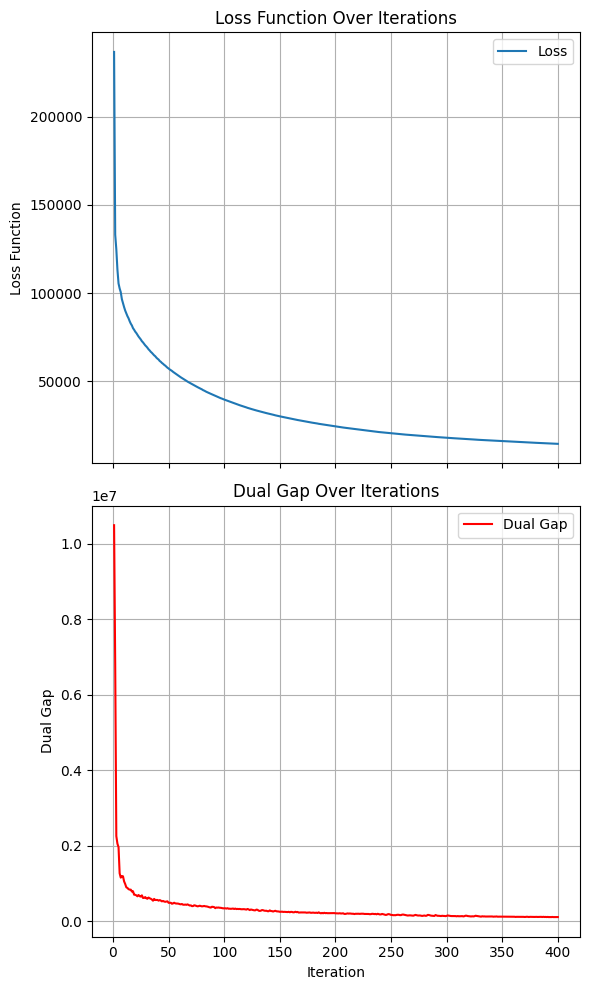
\includegraphics[width=0.8\textwidth]{images/anime_loss_gap}
    \caption{Loss function and dual gap vs iterations for the Anime User Score dataset.}
    \label{fig:anime}
\end{figure}

These results confirm that the diminishing step size strategy leads to lower accuracy compared to the other methods for the same number of iterations. However, it remains the fastest method in terms of computational time. On the other hand, exact line search, while achieving high accuracy, is the slowest method in terms of time. This further supports the argument that adaptive learning rate strategies, particularly Armijo, strike a balance between speed and accuracy, making them more suitable for recommendation system applications.



 
\medskip

\printbibliography % Print bibliography

\end{multicols}% end two-column layout 

\end{document}
 
  















